
\subsection{SampleClean Framework}\label{sec:paradigm}
%While data cleaning can help to fix the data errors, cleaning the entire data is a costly process.Many data-cleaning techniques require human involvement~\cite{DBLP:conf/sigmod/JefferyFH08,DBLP:journals/pvldb/FanLMTY10,DBLP:journals/pvldb/YakoutENOI11,DBLP:journals/pvldb/WangKFF12}, which makes data cleaning even harder to scale to large data.Additionally, recent developments in big data systems, such as Shark~\cite{DBLP:conf/sigmod/XinRZFSS13} and Dremel~\cite{DBLP:journals/pvldb/MelnikGLRSTV10}, allow for increasingly fast aggregations of very large amounts of data. We may be able to reduce sampling error with more efficient querying systems, but we still need a scalable technique to manage data errors.

%In this section, we present \saqpplus, a novel framework that cleans only a sample of data and then processes aggregate queries based on the cleaned sample.
Figure~\ref{fig:arch} illustrates all of the components of our framework.
\saqpplus first creates a random sample of dirty data, and then applies a data-cleaning technique to clean the sample. 
After cleaning the sample, \saqpplus uses the cleaned sample to answer aggregate queries.
\saqpplus gives results that are unbiased which means in expectation the estimates are equal to the query results if the entire dataset was cleaned by the data-cleaning technique.

The \saqpplus framework is independent of how samples are cleaned, and in this paper, we consider data cleaning as a user-provided module. %, and assume that it always gives us correct cleaning results.
Specifically, for each tuple in the sample, the cleaning module corrects the attribute values of the tuple, and estimates the number of duplicates for the tuple from the dirty data.
For example, consider a sample, $S = \{t_1, t_2, \cdots, t_7\}$ of the dirty data in Figure~\ref{fig:example}(a). Figure~\ref{fig:example}(b) shows the corresponding cleaned sample. For the first paper $t_1$, we correct \texttt{pub\_year} from 11 to 2011, correct \texttt{citation\_count} from 18 to 144, and identify two duplicate papers (including $t_1$ itself) in the dirty data.

\subsubsection{Cleaning Value and Condition Errors}
To reduce value errors and condition errors, the data-cleaning technique only needs to clean attribute values in the sample, and we can apply a variety of recently proposed data cleaning techniques to achieve this. 
For example, outlier detection~\cite{hellerstein2008quantitative,DBLP:conf/pervasive/JefferyAFHW06} and rule-based approaches~\cite{fan2012foundations,DBLP:conf/sigmod/DallachiesaEEEIOT13} have been proposed to solve this problem. 
In addition, Fan et al.~\cite{DBLP:journals/pvldb/FanLMTY10} proposed editing rules, master data and user confirmation to correct attribute values, and they proved that their approaches can always obtain perfect cleaning results. There are also some data-cleaning tools~\cite{openrefine,wrangler} that can facilitate users to clean data based on their domain knowledge. 
For example, OpenRefine~\cite{openrefine} allows users to define facets on a per attribute basis, and helps them to quickly identify incorrect attribute values via faceted search.  

\begin{figure}[tup]\centering \vspace{-2em}
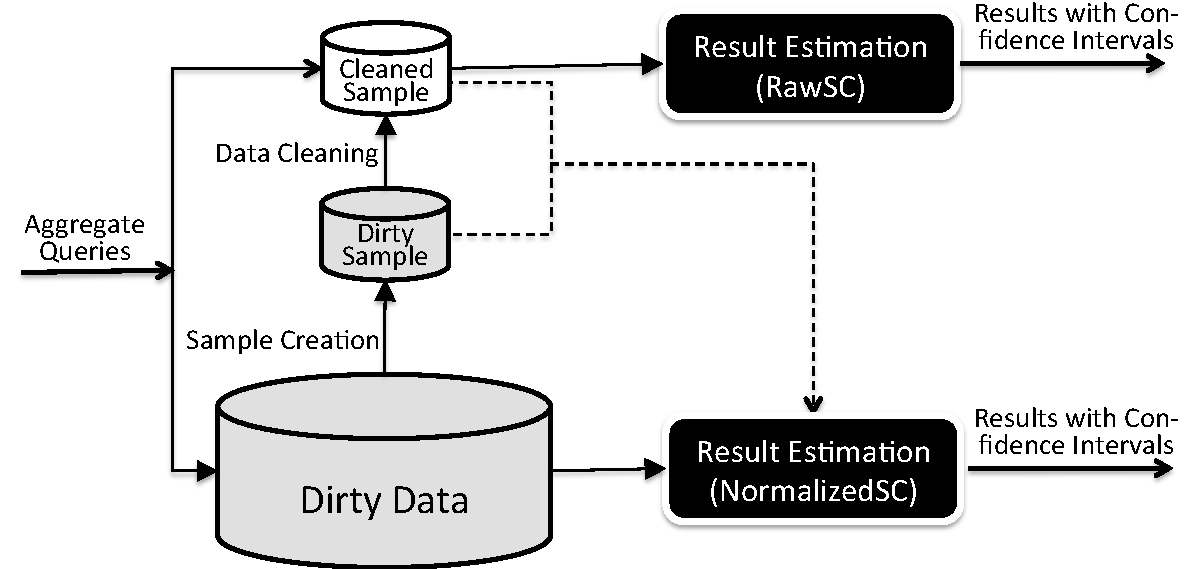
\includegraphics[scale=0.4]{figs/newarch.pdf}
\caption{The \saqpplus framework.}\vspace{-1em}
\label{fig:arch}
%\vspace*{-10pt}
\end{figure}

\subsubsection{Identifying Duplicates}\label{sec:duplication}
\iffalse
The \saqpplus framework defines the duplicate rate for a tuple as the number of times the tuple has been duplicated in the entire table. We cannot, however, achieve an accurate estimate of the duplication rate by only searching in a sample. This method may lead to inaccurate query results, as shown both analytically and empirically in~\cite{charikar2000towards}. Consequently, we must scan the entire table once to obtain the duplicate rate.







\iffalse
Duplicate detection or entity resolution has been extensively studied for several decades~\cite{DBLP:journals/tkde/ElmagarmidIV07}.
\saqpplus needs an estimate of the duplication rate for a tuple which we define as the number of times the tuple has been duplicated in the entire table.
It is known that estimating the duplication rate from only searching in a sample leads to inaccurate query results~\cite{charikar2000towards}.
Consequently, we cannot avoid a scan of the entire table to clean this error type.}
\fi

However, in certain situations, sampling can make duplicate detection more efficient.
The key point is that, we only need to determine the duplication rate for those tuples in our sample. 
To illustrate why, consider the two phases used by most duplicate detection techniques:
\begin{enumerate}\vspace{-.25em}
\item \emph{Blocking}. 
In a pre-processing step, the tuples are coarsely partitioned into small blocks.
This reduces the enormous quadratic cost of all-pairs comparison, and the search can be restricted to within the same block. 
For instance, if we partition \texttt{papers} based on \texttt{conference\_name}, then only the papers that are published in the same conference will be checked for duplicates. 
%Note that we only have to perform blocking once and this can be done offline, e.g., when we are creating the sample. \vspace{-.5em}
%There are many effective techniques for block retrieval such as using a hash index~\cite{journals/tkde/Christen11}.
\item \emph{Matching}. 
To decide whether two tuples are duplicates, some existing techniques model this problem as a classification problem, and train a classifier to label each tuple pair as duplicate or non-duplicate~\cite{DBLP:conf/kdd/BilenkoM03}. 
Other recent work also explores the use of crowdsourcing and asks crowd workers to match tuple pairs~\cite{DBLP:journals/pvldb/WangKFF12,DBLP:conf/www/DemartiniDC12}.
\end{enumerate}\vspace{-.25em}

A recent survey on duplicate detection has argued that the matching phase is typically much more expensive than the blocking phase~\cite{journals/tkde/Christen11}. 
For instance, an evaluation of the popular duplicate detection technique~\cite{DBLP:conf/kdd/BilenkoM03} shows that the matching phase takes on the order of minutes for a dataset of thousands of tuples~\cite{journals/pvldb/KopckeTR10}.
This is especially true in the context of crowdsourced matching where each comparison is performed by a crowd worker costing both time and money.
\saqpplus reduces the number of comparisons in the matching phase, as we only have to match each tuple in the sample with the others in its block.
For example, if we sample 1\% of the table, then we can reduce the matching cost by a factor of 100.



%For duplication errors, the data-cleaning technique only needs to enumerate each tuple in the sample (instead of the entire data), and estimate its duplicates (i.e., those tuples that refer to the same real-world entity as the tuple) from the entire data. 
%This problem is known as duplicate detection or entity resolution, which has been extensively studied for several decades (see~\cite{DBLP:journals/tkde/ElmagarmidIV07} for a survey). 

%Although the blocking phase can be efficiently implemented using a hash index~\cite{journals/tkde/Christen11}, the matching phase is usually much more time-consuming, which either requires sophisticated machine-learning techniques or expensive human-labeling effort. %, thus the cost of deduplication process is typically measured by the number of pair comparisons in the matching phase~\cite{journals/tkde/Christen11}. 
%Consider a data size of $N$ and a sample size of $K$. Assume the average block size is $B$. Without sampling the matching phase has to compare $N\times B$ pairs of tuples. However, with the help of our framework the number is reduced to $K\times B$, which saves the matching cost by $\frac{N}{K}$ times. 
\fi

The \saqpplus framework defines the duplicate factor for a tuple as the number of times the tuple appears in the entire table. To determine it, one way would be to estimate its value from the sample. However, both analytical proofs and empirical tests have shown that this method can lead to highly inaccurate query results~\cite{charikar2000towards}.
Therefore, in our paper, we determine the duplication factor from the complete relation. 



\iffalse
Duplicate detection or entity resolution has been extensively studied for several decades~\cite{DBLP:journals/tkde/ElmagarmidIV07}.
\saqpplus needs an estimate of the duplication rate for a tuple which we define as the number of times the tuple has been duplicated in the entire table.
It is known that estimating the duplication rate from only searching in a sample leads to inaccurate query results~\cite{charikar2000towards}.
Consequently, we cannot avoid a scan of the entire table to clean this error type.}
\fi

It is important to note, however, that compared to full cleaning, we only need to determine the duplication factor for those tuples in the sample. As with other uses of sampling, this can result in significant cost savings in duplicate detection.
In the following, we will describe how to apply existing deduplication techniques to compute the duplication factor, and explain why it is cheaper to determine the duplication factor for a sample of the data, even though doing so requires access to the complete relation.


Duplicate detection (also known as entity resolution) aims to identify different tuples that refer to the same real-world entity. This problem has been extensively studied for several decades (see~\cite{DBLP:journals/tkde/ElmagarmidIV07} for a survey).  
Most deduplication approaches consist of two phases:

\begin{enumerate}\vspace{-.25em}
\item \emph{Blocking}. 
\textit{Due to the large (quadratic) cost of all-pair comparisons, data is partitioned into a number of blocks, and duplicates are considered only within a block. 
For instance, if we partition \texttt{papers} based on \texttt{conference\_name}, then only the papers that are published in the same conference will be checked for duplicates; \vspace{-.25em}}
%Note that we only have to perform blocking once and this can be done offline, e.g., when we are creating the sample.
%There are many effective techniques for block retrieval such as using a hash index~\cite{journals/tkde/Christen11}.
\vspace{-.25em}
\item \emph{Matching}. 
\textit{To decide whether two tuples are duplicates or not, existing techniques typically model this problem as a classification problem, and train a classifier to label each tuple pair as duplicate or non-duplicate~\cite{DBLP:conf/kdd/BilenkoM03}. 
In some recent research (and also at many companies) crowdsourcing is used to get humans to match tuples~\cite{DBLP:journals/pvldb/WangKFF12,DBLP:conf/www/DemartiniDC12}.}
\end{enumerate}\vspace{-.25em}

A recent survey on duplicate detection has argued that the matching phase is typically much more expensive than the blocking phase~\cite{journals/tkde/Christen11}. 
For instance, an evaluation of the popular duplicate detection technique~\cite{DBLP:conf/kdd/BilenkoM03} shows that the matching phase takes on the order of minutes for a dataset of thousands of tuples~\cite{journals/pvldb/KopckeTR10}.
This is especially true in the context of crowdsourced matching where each comparison is performed by a crowd worker costing both time and money.
\saqpplus reduces the number of comparisons in the matching phase, as we only have to match each tuple in the sample with the others in its block.
For example, if we sample 1\% of the table, then we can reduce the matching cost by a factor of 100.

\subsubsection{Result Estimation}



%There are also many studies in dealing with the duplication error (see~\cite{DBLP:journals/tkde/ElmagarmidIV07} for a survey). Particularly, recent work explores the use of crowdsourcing to solve this problem. For example, Wang et al.~\cite{DBLP:journals/pvldb/WangKFF12} proposed a hybrid human-machine framework, which first adopts machine-based techniques to filter obviously non-duplicate tuples for each tuple, and then utilizes the crowd to check the remaining ones.



%For each tuple in the sample, the data-cleaning technique corrects the attribute values of the tuple, and finds the number of duplicates for the tuple from the dirty data. 



After cleaning a sample, \saqpplus uses the cleaned sample to estimate the result of aggregate queries.
Similar to existing \saqp systems, we can estimate query results directly from the cleaned sample. However, due to data error, result estimation can be very challenging. For example, consider the $\avgfunc(\texttt{citation\_count})$ query in previous section. Assume that the data has duplication errors and that papers with a higher citation count tend to have more duplicates. The greater the number of duplicates, the higher probability a paper is sampled, and thus the cleaned sample may contain more highly cited papers, leading to an over-estimated citation count. We formalize these issues and propose the \sampleclean approach to address them in Section~\ref{sec:sampleclean}.




Another quantity of interest is how much the dirty data differs from the cleaned data. 
We can estimate the mean difference based on comparing the dirty and cleaned sample, and then correct a query result on the dirty data with this estimate. We describe this alternative approach, called \biascorrected, and compare its performance with \sampleclean in Section~\ref{sec:biascorrected}.

\iffalse
\vspace{.5em}
{\noindent \bf An Example Implementation:} We will walk through an example implementation of SampleClean using OpenRefine~\cite{openrefine} to clean the data. 
Consider our example dirty dataset of publications in Figure~\ref{fig:example}(a).  
First, the user creates a sample of 100 records and loads this sample into the OpenRefine spreadsheet interface.
The user can use the tool to detect data errors such as missing attributes, and fill in the correct values (e.g., from another source or based on prior domain expertise).
Next, for deduplication, the system will propose potential matches for each publication in the sample based on a blocking technique %(e.g., locality sensitive hashing of the titles)
and the user can accept or reject these matches.
Finally, the clean sample with the deduplication information is loaded back into the dataset.
To query this clean sample, we need to apply \saqpplus's result estimation to ensure that the estimate remains unbiased after cleaning as some records may have been removed, corrected, or marked as duplicates. 

In this example, sampling significantly reduces the data cleaning effort for the user. 
The user needs to inspect only 100 records instead of the entire dataset, and has no more than 100 sets of potential duplicates to manually check.
In the rest of the paper, we discuss the details of how to ensure unbiased estimates, and how large the sample needs to be to get a result of acceptable quality.
\fi

\vspace{.5em}
{\noindent \bf \saqpplus v.s. \saqp:} \saqp assumes perfectly clean data while \saqpplus relaxes this assumption and makes cleaning feasible.
In \sampleclean, we take a sample of data, apply a data cleaning technique, and then estimate the result.
The result estimation is similar to \saqp, however, we require a few additional scaling factors related to the cleaning.
On the other hand, \bias is quite different from typical \saqp frameworks.
\bias estimates the average difference between the dirty and cleaned data, and this is only possible in systems that couple data cleaning and sampling. 
What is surprising about SampleClean is
that sampling a relatively small population of the overall data makes
it feasible to manually or algorithmically clean the sample, and
experiments confirm that this cleaning often more than compensates for
the error introduced by the sampling.
%Existing \saqp systems can process queries on a dirty sample, and the query results will contain both sampling error and data error.
%Since \saqpplus estimates from a cleaned sample, its results will have reduced data error.
%When the reduction in data error is greater than the sampling error, \saqpplus will give results more accurate than the aggregation of the entire dataset.

\subsubsection{Example: Publication Cleaning with OpenRefine}
In this section, we will walk through an example implementation of SampleClean using OpenRefine~\cite{openrefine} to clean the data. 
Consider our example dirty dataset of publications in Figure~\ref{fig:example}(a). %, and our example aggregate query that calculates the average citations received per publication grouped by the year. %\reminder{I suggest not to show the query before you clean a sample. It looks like sample creation and data cleaning are related to the given query.} 
First, the user creates a sample of data (e.g., 100 records) and loads this sample into the OpenRefine spreadsheet interface.
The user can use the tool to detect data errors such as missing attributes, and fill in the correct values (e.g., from another data source or based on prior domain expertise).
Next, for deduplication, the system will propose potential matches for each publication in the sample based on a blocking technique %(e.g., locality sensitive hashing of the titles)
and the user can accept or reject these matches.
Finally, the clean sample with the deduplication information is loaded back into the dataset. In this example, sampling reduces the data cleaning effort for the user. 
The user needs to inspect only 100 records instead of the entire dataset, and has no more than 100 sets of potential duplicates to manually check.


To query this clean sample, we need to apply \saqpplus's result estimation to ensure that the estimate remains unbiased after cleaning since some records may have been corrected, or marked as duplicates. 
%For instance, in our example aggregate query that calculates the average citations received per publication grouped by the year, if publications from some years were more likely to be duplicated that could introduce a bias into a result estimate.
In the rest of the paper, we discuss the details of how to ensure unbiased estimates, and how large the sample needs to be to get a result of acceptable quality.


%To facilitate a flexible trade-off between data-cleaning cost and answer quality, \saqpplus also allows users to specify a result-quality or cleaning-cost constraint for their aggregate queries. For example, users may want to know that given a cleaning budget, what is the best result quality they can achieve? Or, given a quality constraint, how many samples they need clean to meet the constraint? We discuss how to address these problems in Section~\ref{sec:query-processing}.


%After obtaining the estimate results using \sampleclean and \biascorrected, \saqpplus compares the sizes of their confidence intervals, and returns the result with a narrower confidence interval. In addition, \saqpplus also allows users to specify a result-quality or cleaning-cost constraint for their queries. For example, users may require the confidence interval should be no larger than a threshold. In this case, \saqpplus will check whether the current result satisfies the constraint. If not, it will request to clean more data until the confidence interval satisfies the threshold. 

%While data cleaning can help to fix the data errors, cleaning the entire data is a costly process.
%Many data-cleaning techniques require human involvement~\cite{DBLP:conf/sigmod/JefferyFH08,DBLP:journals/pvldb/FanLMTY10,DBLP:journals/pvldb/YakoutENOI11,DBLP:journals/pvldb/WangKFF12}, which makes data cleaning even harder to scale to big data.

%To this end, we propose \saqpplus, a novel framework by integrating sampling with data cleaning for processing aggregate queries. 
%We first present an overview of \saqpplus framework in Section~\ref{subsec:new-paradigms}, and then discuss two key characteristics about our framework in Section~\ref{subsec:characteristics}.

%While data cleaning can help to fix the data errors, it is a very costly process, and hard to scale to large data.  
%In this section, we explore to integrate sampling with data cleaning. We first present \saqpplus framework based on this idea in Section~\ref{subsec:new-paradigms}, and then discuss two key characteristics about our framework in Section~\ref{subsec:characteristics}.



\iffalse
\subsection{Overview}\label{subsec:new-paradigms}
%Existing \saqp systems are  able to provide a flexible trade-off between sampling error and query response time. However, sampling error may not be the biggest challenge in big data queries.
%In practice, the data itself may contain errors, and even running a query on the entire data, let alone a sample, may still lead to arbitrarily erroneous results. 
%While data cleaning can help to fix the data errors, cleaning the entire data is a costly process.
%Many data-cleaning techniques require human involvement~\cite{DBLP:conf/sigmod/JefferyFH08,DBLP:journals/pvldb/FanLMTY10,DBLP:journals/pvldb/YakoutENOI11,DBLP:journals/pvldb/WangKFF12}, which makes data cleaning even harder to scale to big data. To this end, we propose \saqpplus, a scalable framework to manage data errors which targets at achieving a flexible trade-off between cleaning cost and result quality.
As shown in Figure~\ref{fig:arch}, \saqpplus first creates a random sample of the data, and then applies a data-cleaning technique to clean the sample. Given an aggregate query, \saqpplus employs two estimation approaches to obtain its query result. \biascorrected estimates how data error affects the query result based on the cleaned sample, and  corrects the result's bias on the entire data. \sampleclean directly estimates the query result based on the cleaned sample without accessing the entire data. Both \biascorrected and \sampleclean can obtain unbiased query results along with confidence intervals.

After obtaining the estimate results using \sampleclean and \biascorrected, \saqpplus compares the sizes of their confidence intervals, and returns the result with a narrower confidence interval. In addition, \saqpplus also allows users to specify a result-quality or cleaning-cost constraint for their queries. For example, users may require the confidence interval should be no larger than a threshold. In this case, \saqpplus will check whether the current result satisfies the constraint. If not, it will request to clean more data until the confidence interval satisfies the threshold. 




\subsection{Characteristics}\label{subsec:characteristics}
In this section, we discuss two key characteristics about \saqpplus framework: The first one shows that \saqpplus can provide a better trade-off between cleaning cost and result quality (Section~\ref{subsubsec:trade-off}); The second one indicates that \saqpplus with only \sampleclean  may achieve both lower latencies and better quality than running queries over the entire dirty data (Section~\ref{subsubsec:less-more}).



\subsubsection{Cleaning cost v.s. result quality trade-off}\label{subsubsec:trade-off}
%We use a real-world data to illustrate our idea. We crawled the papers of Rakesh Agarwal from his author profile at Microsoft Academic Search. 

%We illustrate our idea with a real experimental result (see Section~\ref{exp:mas} for more details). We crawled all the papers of Rakesh Agarwal from Microsoft citation index. Due to data errors, some papers are not written by him and some papers are duplicate. After cleaning all  of these papers, we can get his real paper count. In Figure~\ref{fig:tradeoff}, we varied the number of cleaned papers, and compared the error of his paper counts returned by \saqpplus and \alldirty and \allclean, where \alldirty does not clean any paper and \allclean cleans all the papers.
\begin{figure}[tup]\centering
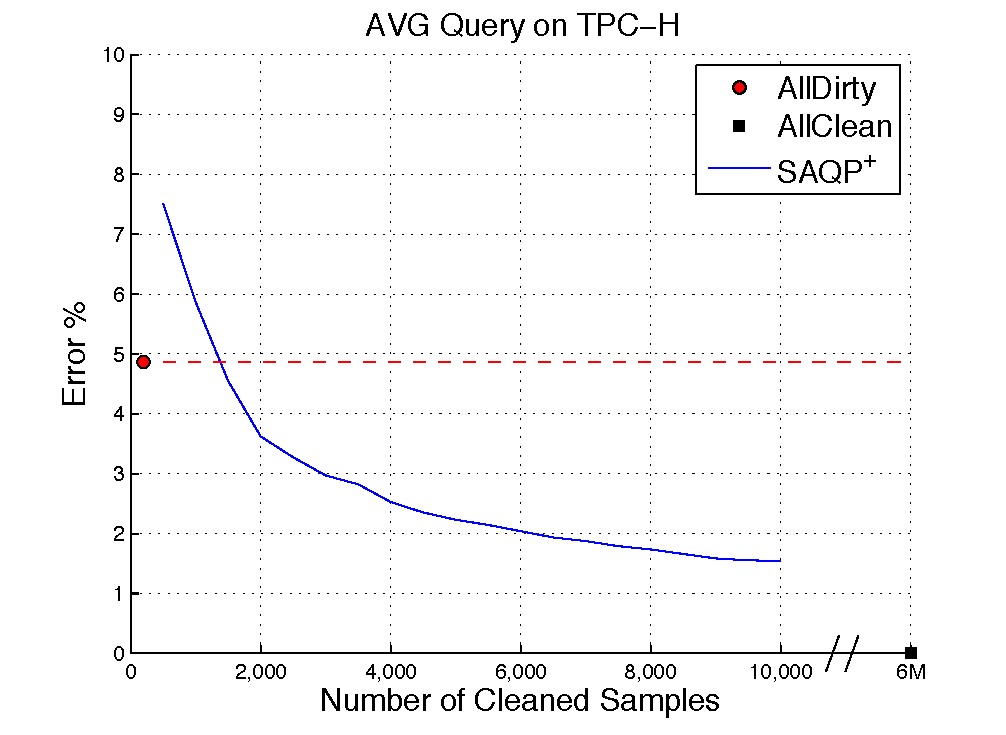
\includegraphics[scale=0.35]{figs/tradeoff-new.pdf}
\caption{Cleaning cost v.s. result quality trade-off.}
\label{fig:tradeoff}
\end{figure}

We illustrate the first characteristic with a real experimental result. We ran an average query on a 1GB \mbox{TPC-H} dataset with 3\% aggregation, 1\% predicate and 2\% duplication errors (see Section~\ref{exp:tpch} for more details). After cleaning all of the data (i.e., more than 6 million tuples), we can get the true query result. In Figure~\ref{fig:tradeoff}, we varied the number of cleaned tuples, and compared the error of query results returned by \saqpplus and \alldirty and \allclean, where \alldirty (\allclean) represents the approach that cleans none (all) of the data.


%As shown in Figure~\ref{fig:tradeoff}, \saqpplus gradually converges to \allclean by cleaning more and more data. This is because with the increase of cleaned sample size, \biascorrected and \sampleclean can be more accurate in  estimating the data error and the \allclean's result, respectively. After cleaning the entire data, both of them will be equivalent to \allclean. 


As shown in Figure~\ref{fig:tradeoff}, \saqpplus can obtain very good results by only cleaning a few tuples. For instance, \saqpplus outperforms \alldirty when the number of cleaned samples is larger than 1500 (0.025\% of 6M tuples). With more samples cleaned, \saqpplus can achieve better and better results until reaching \allclean that needs to clean all the data. Therefore, \allclean is only a special case of \saqpplus, and \saqpplus provides a better quality/cost trade-off than both \alldirty and \allclean. 


%In comparison with \alldirty, \saqpplus can outperform \alldirty when the cleaned sample size is larger than 1500.
%More importantly, \saqpplus returns an unbiased query result with the quality guarantee, and users can easily adjust the result quality by cleaning more or less data. But \alldirty simply returns a query result with no quality guarantee, which could be arbitrarily erroneous and hard to make users trust even if it is very accurate.



\subsubsection{Less can be more}\label{subsubsec:less-more} 
While sampling can make query processing more efficient, people commonly believe running queries on a sampled data is less accurate than obtaining results from the entire data. However, when the data is dirty, we have an interesting observation that \sampleclean, which directly estimates results from the cleaned sample, can even achieve better quality than \alldirty. This is because \sampleclean only involves sampling error while \alldirty has data errors. The more the number of cleaned samples, the less sampling error. When the sampling error becomes less than the data error, \sampleclean outperforms \alldirty. This surprising observation implies that \saqpplus with only \sampleclean may achieve both lower latencies and better quality than \alldirty. 



\fi
 
